\documentclass[12pt]{article}

\usepackage{fullpage}
\usepackage[spanish]{babel}
\usepackage{amsfonts} %for double trace letters
\usepackage{amssymb}
\usepackage{amsmath} %for special/unusual mathematical characters
\usepackage{mathrsfs} % For curly letters
\usepackage{eufrak} %for gothic letters
\usepackage{graphicx} %Image includer package
\graphicspath{{Images/}} %Image directory
\usepackage{xcolor}
\usepackage{esint} % for simple counter-clockwise directed contour integral symbol

% For loops
\usepackage{forloop}
\usepackage{pgffor}

% For index
\usepackage[utf8]{inputenc}
\usepackage{imakeidx}
\usepackage{hyperref}% for hyperlinked index
\makeindex

% For table of contents with links to section
\usepackage{hyperref}
\hypersetup{
    colorlinks=true, %set true if you want colored links
    linktoc=all,     %set to all if you want both sections and subsections linked
    linkcolor=black,  %choose some color if you want links to stand out
}

\usepackage{multicol} %For writing text in columns
\setlength{\columnsep}{1cm} %Defines separation of columns

\usepackage{tcolorbox} %for boxes that enclose text
\usepackage{color}
\definecolor{myblue}{rgb}{.8, .8, 1}

\usepackage{empheq}

%for green eq box
%\definecolor{lightgreen}{HTML}{90EE90}
%\newcommand{\boxedeq}[2]{\begin{empheq}[box=\colorbox{lightgreen}]{align}\label{#1}#2\end{empheq}}

%for blue eq box
\newlength\mytemplen
\newsavebox\mytempbox

\makeatletter
\newcommand\mybluebox{%
    \@ifnextchar[%]
       {\@mybluebox}%
       {\@mybluebox[0pt]}}

\def\@mybluebox[#1]{%
    \@ifnextchar[%]
       {\@@mybluebox[#1]}%
       {\@@mybluebox[#1][0pt]}}

\def\@@mybluebox[#1][#2]#3{
    \sbox\mytempbox{#3}%
    \mytemplen\ht\mytempbox
    \advance\mytemplen #1\relax
    \ht\mytempbox\mytemplen
    \mytemplen\dp\mytempbox
    \advance\mytemplen #2\relax
    \dp\mytempbox\mytemplen
    \colorbox{myblue}{\hspace{1em}\usebox{\mytempbox}\hspace{1em}}}

% For arrow comment
\usepackage{tikz}
\usetikzlibrary{tikzmark,arrows,calc}
\newcommand\sidecomment[5][0.3,0.1]%
  {\begin{tikzpicture}[remember picture,overlay]
   \draw[-stealth',thick]
     ($({pic cs:#4}|-{pic cs:#2})+(#1)$)
     .. controls +(1,0) and +(1,0) ..
     node[right,align=left]{#5}
     ($({pic cs:#4}|-{pic cs:#3})+(#1)$);
   \end{tikzpicture}%
  }

% for theorems
\usepackage{amsthm}
 
\theoremstyle{definition}
\newtheorem{definition}{Definici\'on}[section]

\theoremstyle{theorem}
\newtheorem{theorem}{Teorema}[section]

\theoremstyle{corolary}
\newtheorem{corolary}{Corolario}[section]

\theoremstyle{method}
\newtheorem{method}{Regla}

\DeclareMathOperator{\Arg}{Arg}
\DeclareMathOperator{\Log}{Log}
\DeclareMathOperator{\sen}{sen}
\DeclareMathOperator{\senh}{senh}
\DeclareMathOperator{\tg}{tg}
\DeclareMathOperator{\ctg}{ctg}
\DeclareMathOperator{\tgh}{tgh}
\DeclareMathOperator{\ctgh}{ctgh}
\DeclareMathOperator{\sech}{sech}
\DeclareMathOperator{\csch}{csch}
\DeclareMathOperator*{\Res}{Res}


\begin{document}
	\title{La Transformada de Laplace}
	\author{Breggia, Bruno M.}
	\date{}
	\maketitle

\ \\

\begin{center}
	
\includegraphics[scale=0.6]{El_mundo.png}
\end{center}

\ \\

?`Qu\'e tanto nos pueden predecir las matem\'aticas? Aqu\'i les presentaremos la muy revolucionadora \textbf{Transformada de Laplace}, elemento important\'isimo en el an\'alisis de se\~nales y sistemas, y por dem\'as \'util en modelar f\'isicamente al Universo, brind\'andonos de un medio por el cual predecir fen\'omenos y comportamientos...


\pagebreak

\section{La utilidad de la herramienta}
La Transformada de Laplace es una potente herramienta matem\'atica que juega un rol clave en:
\begin{itemize}
	\item An\'alisis y dise\~no de sistemas de ingenier\'ia
	\item Resoluci\'on de ecuaciones diferenciales lineales mediante la transformaci\'on en ecuaciones algebraicas
	\item Estudio de se\~nales y sistemas (sistemas mec\'anicos, circuitos el\'ectricos)
	\item Sistemas de control
\end{itemize}

\section{Integrales impropias}
Antes de adentrarnos a lo m\'as interesante, la transformada de Laplace, recalcaremos el importante concepto de integral impropia, ya ver\'an por qu\'e.\\

\colorbox{violet!40!white!80}{\parbox{\linewidth}{
\theoremstyle{definition}
\begin{definition}{Integral Impropia}

Sea $f:[a,b]\to \mathbb{R}\ \acute{o}\ \mathbb{C}$ una funci\'on de variable real a valores reales o complejos. Entonces $$\int\limits_a^b f(t)\ dt$$ ...se define bajo las siguientes condiciones:

\begin{itemize}
	\item $\mbox{Dom}(f)$ es un conjunto acotado
	\item $f$ est\'a acotada en el intervalo $[a,b]$
\end{itemize}

Si alguna de estas condiciones \textit{no} se cumple, denominaremos a la integral como \textbf{integral impropia}.

\end{definition}}}
\linebreak
\linebreak

Tenemos entonces dos condiciones que si se violan, nos dan lugar a las integrales impropias. Acorde a cu\'al regla se viole, tendremos una integral impropia de primera o segunda especie:

\begin{itemize}
	\item Sea $f:[a, \infty) \to \mathbb{R}\ \acute{o} \ \mathbb{C}$ integrable en $[a,\varepsilon]\ \forall\varepsilon \geq a $.\\
	Si {\color{red} Dom($f$) no es un conjunto acotado}, entonces se dice que la integral impropia  $\int\limits_a^{+\infty}f(t)\ dt$ es de \textbf{primera especie} s\'olo si converge (o existe) el l\'imite $$\lim\limits_{\varepsilon\to +\infty} \int\limits_a^{\varepsilon}f(t)\ dt$$
	\item Sea $f:(a,b] \to \mathbb{R}\ \acute{o} \ \mathbb{C}$ integrable en $[\varepsilon,b]\ \forall\varepsilon\in (a,b]$.\\
	Si {\color{red} $f$ no est\'a acotada en $a$}, entonces se dice que la integral impropia  $\int\limits_{a^+}^b f(t)\ dt$ es de \textbf{segunda especie} s\'olo si converge (o existe) el l\'imite $$\lim\limits_{\varepsilon\to a^+} \int\limits_{\varepsilon}^b f(t)\ dt$$
	
\end{itemize}

\colorbox{violet!40!white!80}{\parbox{\linewidth}{
\theoremstyle{definition}
\begin{definition}{Convergencia}

Sea $f(t)$ una funci\'on de la variable real $t\in [0, \infty)\to \mathbb{R}\ \acute{o}\ \mathbb{C}$, continua o con una cantidad finita de discontinuidades de salto finito.

Se dice que la integral impropia $\int\limits_0^{+\infty} f(t)\ dt$ \textbf{converge} (o \textbf{existe}) cuando:
\begin{itemize}
	\item Para el caso en que Dom($f$) no est\'e acotado, si existe el l\'imite: $$\lim\limits_{b\to\infty} \int\limits_0^b f(t)\ dt$$
	\item Para el caso en que $f(t)$ no est\'a acotada en $t=0$, si existe el l\'imite: $$\lim\limits_{\varepsilon\to 0^+}f(t)\ dt$$
\end{itemize}

\end{definition}}}
\linebreak
\linebreak

\section{Una f\'ormula para dominarlos a todos}

No esperen m\'as. A continuaci\'on, la definici\'on de la Transformada de Laplace. Pero antes cabe recalcar, de ahora en m\'as se har\'a un \textit{peque\~no} cambio en la notaci\'on: la unidad imaginaria ser\'a \textbf{j}, y no la \textit{i} de imaginario, por cuestiones ingenieriles (en este nuevo contexto, la \textit{i} suele representar corriente el\'ectrica, y no nos queremos confundir).\\

\colorbox{red!40!white!80}{\parbox{\linewidth}{
\theoremstyle{definition}
\begin{definition}{La Transformada de Laplace}

Sea $f(t)$ una funci\'on de la variable real $t\in[0,\infty)\to \mathbb{R}\ \acute{o} \ \mathbb{C}$ continua o seccionalmente continua.
Sea $s = \sigma + j\omega \in \mathbb{C}$.

Si existe la integral impropia $\int_0^{+\infty}f(t) e^{-st}\ dt$ para ciertos valores de $s$, se dice que dicha integral es la \textbf{Transformada de Laplace} de $f(t)$, y se indica: $$\mathscr{L}\{f(t)\} = \int\limits_0^{+\infty}f(t)\ e^{-st}\ dt$$

El conjunto de valores para los cuales converge la integral se denomina \textbf{regi\'on de convergencia} de la transformada.
\end{definition}}}
\linebreak
\linebreak

A $\mathscr{L}\{\cdot\}$ se lo denomina \textbf{Operador Transformada de Laplace} de $f(t)$ y se escribe: $$F(s) = \mathscr{L}\{f(t)\}$$ siendo $F(s)$ la \textbf{Transformada de Laplace} de $f(t)$.

Este operador transforma una funci\'on de dominio de tiempo $t$ en una funci\'on de dominio de frecuencia compleja $s$. Es una de toda una familia de \textbf{transformaciones integrales}: $$\mathscr{T}\{f(t)\} = \int\limits_a^b K(u,t)\ f(t)\ dt = F(u)$$

\subsection*{Desglosando el operador $\mathscr{L}\{\cdot\}$}
\ \\
$$F(s) = \mathscr{L}\{f(t)\} = \int\limits_0^{+\infty}f(t)\ e^{-st}\ dt$$
\ \\
\begin{itemize}
	\item $f(t)$ es una \textbf{funci\'on} continua o seccionalmente continua en el tiempo, definida en $[0, +\infty)$
	\item $\mathscr{L}\{f(t)\}$ es el \textbf{operador} transformada de Laplace
	\item $e^{-st}$ es el \textbf{n\'ucleo} de la Transformaci\'on
	\item $s$ es la variable que representa la \textbf{frecuencia compleja} ($s\in \mathbb{C}$)
	\item $F(s)$ es la \textbf{Transformada de Laplace} de $f(t)$
\end{itemize}

\subsection*{Funciones elementales}
A continuaci\'on una tabla con las transformadas de Laplace de funciones elementales

{\large
\begin{center}
\begin{tabular}{c|c|c}
$f(t)$ & $\qquad F(s) \qquad$ & Regi\'on de Convergencia\\
\hline
&&\\
$c$ & $\displaystyle\frac{c}{s}$ & $\mathfrak{Re}(s)>0$\\
&&\\
$t$ & $\displaystyle\frac{1}{s^2}$ & $\mathfrak{Re}(s)>0$\\
&&\\
$t^n$ & $\displaystyle\frac{n!}{s^{n+1}}$ & $\mathfrak{Re}(s)>0$\\
&&\\
$e^{at}$ & $\displaystyle\frac{1}{s-a}$ & $\mathfrak{Re}(s)>\mathfrak{Re}(a)$\\
&&\\
$\cos(at)$ & $\displaystyle\frac{s}{s^2+a^2}$ & $\mathfrak{Re}(s)>|\mathfrak{Im}(a)|$\\
&&\\
$\sen(at)$ & $\displaystyle\frac{a}{s^2+a^2}$ & $\mathfrak{Re}(s)>|\mathfrak{Im}(a)|$\\
&&\\
$\cosh(at)$ & $\displaystyle\frac{s}{s^2-a^2}$ & $\mathfrak{Re}(s)>|\mathfrak{Re}(a)|$\\
&&\\
$\senh(at)$ & $\displaystyle\frac{a}{s^2-a^2}$ & $\mathfrak{Re}(s)>|\mathfrak{Re}(a)|$\\
\end{tabular}
\linebreak
\end{center}
}

%$\mathscr{L}$

\subsection*{La Transformada Bilateral}
Si te quedaste inc\'omodo pensando por qu\'e la transformada es una integral que parte de 0 hasta infinito y no desde infinito negativo, esta nueva definici\'on te dejar\'a satisfecho.\\

\colorbox{red!40!white!80}{\parbox{\linewidth}{
\theoremstyle{definition}
\begin{definition}{La Transformada Bilateral de Laplace}

Si $f(t)$ est\'a definida para todo $t\in \mathbb{R}$, se define la \textbf{Transformada de Laplace Bilateral} como: $$\mathscr{L}_B\{f(t)\} = F(s) = \int\limits_{-\infty}^{+\infty}f(t)\ e^{-st}\ dt $$

si se da que dicha integral impropia existe.
\end{definition}}}
\linebreak
\linebreak


\colorbox{yellow!40!white!80}{\parbox{\linewidth}{
\theoremstyle{definition}
\begin{definition}{Funci\'on causal}

Si $f(t)$ est\'a definida para todo $t\in \mathbb{R}$, se dice que es una funci\'on causal si $f(t)=0$ para todo $t<0$.
\end{definition}}}
\linebreak
\linebreak

Esta definici\'on de funci\'on causal nos viene a dar la idea de que trataremos con funciones, o \textit{se\~nales}, que modelar\'an fen\'omenos con respecto al tiempo, el cual no tiene valor alguno en instantes por detr\'as del 0 (?`o alguna vez programaron alguna cita en tiempo negativo?). Por ello, en cualquier valor negativo, la funci\'on vale cero. Usando precisamente este tipo de funciones, con una $f(t)$ causal, tenemos: $$\mathscr{L}_B\{f(t)\} = \mathscr{L}\{f(t)\} = \int\limits_{0}^{+\infty}f(t)\ e^{-st}\ dt $$

\subsection*{Condiciones Suficientes}

Hablemos ahora de algo que nos deber\'ia incumbir, y que quiz\'as no le hayan dado mucha importancia, pero que no por ello deja de ser esencial... ?`toda funci\'on causal en el dominio de tiempo real tiene una transformada de Laplace en el dominio de frecuencia compleja? Hemos visto anteriormente que hay valores restringidos de $s\in \mathbb{C}$ para los cuales se cumple que la transformada es igual a la expresi\'on $F(s)$. Esto es clara indicaci\'on de que no es aplicable para todo complejo. Y en caso de que no exista n\'umero complejo alguno que nos permita elaborar tal transformada, diremos entonces que \textit{no existe} la transformada de Laplace para la funci\'on $f(t)$ dada.

Diremos entonces que la Transformada de Laplace de $f(t)$ existe si y s\'olo si la integral impropia de la definici\'on converge para al menos algunos valores de $s\in \mathbb{C}$. Esto est\'a, en parte, relacionado con el acotamiento de la funci\'on $f(t)$, con el factor $e^{-st}$ en el n\'ucleo de la transformada actuando como factor de convergencia en que los valores permitidos de $\mathfrak{Re}(s)$ son aquellos para los que la integral converge.

Entonces, antes de introducir condiciones suficientes sobre $f(t)$ para la existencia de $\mathscr{L}\{f(t)\}$, introducimos una nueva definici\'on:


\colorbox{blue!40!white!80}{\parbox{\linewidth}{
\theoremstyle{definition}
\begin{definition}{Funciones de Orden Exponencial}

Una funci\'on $f(t)$ es de \textbf{orden exponencial} cuando $t\to \infty$ si existen un n\'umero real $\sigma$ y constantes reales positivas $M$ y $T$ tales que: $$|f(t)| < Me^{\sigma t}, \qquad \forall t > T$$
\end{definition}}}
\linebreak

Lo que nos dice esta definici\'on es que una funci\'on $f(t)$ es de orden exponencial si no crece m\'as r\'apido que una funci\'on exponencial de la forma $Me^{\sigma t}$.\\

\textbf{Ejemplo 1.} La funci\'on $f(t)=e^{3t}$ es de orden exponencial con $\sigma \geq 3$.\\

\textbf{Ejemplo 2.} Se verificar\'a si $f(t)=t^3$ para $t\geq 0$ es de orden exponencial. Dado que $$e^{\alpha t} = 1 + \alpha t + \frac{1}{2}\alpha^2 t^2 + \frac{1}{6} \alpha^3 t^3 + ...$$ para cualquier $\alpha > 0$, entonces se tiene que $$t^3 < \frac{6}{\alpha^3}\ e^{\alpha t}$$ As\'i que $f(t)=t^3$ es de orden exponencial con $\sigma > 0.$\\

\textbf{Ejemplo 3.} La funci\'on $f(t) = e^{t^2}$ no es de orden exponencial, ya que crece m\'as r\'apidamente que $Me^{\sigma t}$ cuando $t\to \infty$ cualesquiera sean los valores de $M$ y $\sigma$.\\

En los ejemplos anteriores, los valores de $\sigma$ que hemos hallado son en realidad los m\'inimos valores que podr\'ia tomar $\sigma$ para que la funci\'on en cuesti\'on se encuentre acotada por la funci\'on exponencial $Me^{\sigma t}$. Nos interesa precisamente el menor sigma posible, porque tenemos de esta manera, con el $M$ que m\'as nos convenga, lo que denominaremos \textbf{abscisa de convergencia} $\sigma_c$, el cual viene a ser la m\'axima cota inferior del conjunto de valores posibles de $\sigma$.

%\def\b{3}
%\if\b 3
%Hi there \b
%\else
%Bye \b
%\fi

%\newcounter{loop}
%\forloop{loop}{1}{\value{loop}<11}{Hello there\\}

%\newcounter{sum}
%\foreach \n in {1, 2, 3.14} {Hi there: \n \\}

Entonces, en el primer ejemplo $\sigma_c=3$, en el segundo ejemplo $\sigma_c=0$, y en el tercero simplemente $\nexists\ \sigma_c$.

Ya con las herramientas necesarias, concluimos esta secci\'on con el siguiente Teorema de Existencia de la Transformada de Laplace:\\

\colorbox{orange!40!white!80}{\parbox{\linewidth}{
\theoremstyle{theorem}
\begin{theorem} {Existencia de la Transformada de Laplace}\\

Si la funci\'on causal $f(t)$ es continua a trozos en $[0, +\infty)$ y es de orden exponencial con abscisa de convergencia $\sigma_c$, entonces existe la transformada de Laplace con regi\'on de convergencia $\mathfrak{Re}(s)> \sigma_c$ en el dominio complejo. Esto es: $$\mathscr{L}\{f(t)\} = F(s) = \int\limits_0^{+\infty} e^{-st}\ f(t)\ dt, \qquad \mathfrak{Re}(s )> \sigma_c$$
\end{theorem}}}
\linebreak
\linebreak

\texttt{NOTA:} este teorema nos brinda \textit{condiciones suficientes, no necesarias} para la existencia de la transformada de Laplace. Es decir, si se cumplen las condiciones para $f(t)$, entonces posee transformada de Laplace. Pero si \textit{no} las cumple, esto no quiere decir que no posee Transformada. Puede no cumplir con estas condiciones y aun as\'i poseer una transformada de Laplace para cierta regi\'on de convergencia en el plano complejo.

\pagebreak
\section*{Propiedades de la Transformada}
Sinceramente, no vamos a estar como monos calculando la transformada de Laplace de $f(t)$ siempre a partir de la definici\'on... eso ser\'ia calcular muchas integrales, calcular l\'imites, y encima imponer las restricciones necesarias sobre $s\in \mathbb{C}$ para conocer d\'onde converge la transformada obtenida. Y si en el camino te quedas trabado en medio de la nada, habr\'ias encontrado una brusca manera de darte cuenta de que la funci\'on $f(t)$ simplemente no posee transformada de Laplace.

Es por esto que a la Transformada de Laplace se la estudia como un operador de funciones con sus propias propiedades de c\'alculo, que nos permitir\'an calcular la transformada de funciones complicadas a partir del conocimiento de la transformada de funciones m\'as elementales. T\'omense estas propiedades como sus mandamientos, y todo saldr\'a bien...\\

Las propiedades a tratar ser\'an:
\begin{itemize}
	\item Linealidad
	\item Primer Teorema de la Traslaci\'on
	\item Derivada de la transformada
	\item Transformada de la derivada
	\item Transformada de la integral
\end{itemize}

\subsection*{Linealidad}

Por definirse en t\'erminos de una integral, la transformada hereda de ella la propiedad de linealidad.\\

\textit{Si $f(t)$ y $g(t)$ son funciones que poseen transformadad de Laplace para $\mathfrak{Re}(s)>\sigma_{c1}$ y $\mathfrak{Re}(s)>\sigma_{c2}$ respectivamente, con $\alpha$ y $\beta$ constantes cualesquiera, entonces:}

\begin{empheq}[box={\mybluebox[5pt]}]{equation*}
		\mbox{ \large $\mathscr{L}\{\alpha f(t) + \beta g(t)\} = \alpha \mathscr{L}\{f(t)\} + \beta \mathscr{L}\{g(t)\},\qquad \mathfrak{Re}(s)> \max(\sigma_{c1}, \sigma_{c2}) $}
	\end{empheq}

//Demostrar

\subsection*{Primer Teorema de la Traslaci\'on}
El primer teorema de la traslaci\'on, tambi\'en conocida como \textbf{Teorema de la Modulaci\'on Exponencial}, viene dado por:\\

\textit{Si $f(t)$ es una funci\'on que tiene una transformada de Laplace $F(s)$, con $\mathfrak{Re}(s)>\sigma_c$, entonces la funci\'on $e^{at}f(t)$ tambi\'en tiene una transformada de Laplace dada por:}

\begin{empheq}[box={\mybluebox[5pt]}]{equation*}
		\mbox{ \large $\mathscr{L}\{e^{at}f(t)\} = F(s-a), \qquad \mathfrak{Re}(s)>\sigma_c + \mathfrak{Re}(a) $}
	\end{empheq}

//Demostrar

\subsection*{Derivada de la Transformada}
Esta propiedad es una muy potente, que relaciona operaciones en el dominio de tiempo $t$ con aquellas en el dominio transformado $s$. Es conocida tembi\'en como la propiedad de la \textbf{multiplicaci\'on por $t$}. A continuaci\'on su enunciado:\\

\textit{Si $f(t)$ es una funci\'on cuya transformada de Laplace es $F(s)=\mathscr{L}\{f(t)\}$ con $\mathfrak{Re}(s)>\sigma_c$, entonces la funci\'on $t^nf(t)$, para $n=1, 2, 3,...$ tambi\'en tiene transformada de Laplace dada por:}

\begin{empheq}[box={\mybluebox[5pt]}]{equation*}
		\mbox{ \large $\mathscr{L}\{t^n f(t)\} = (-1)^n\ \frac{d^n F(s)}{ds^n}, \qquad \mathfrak{Re}(s)>\sigma_c $}
	\end{empheq}

//Demostrar

\subsection*{Transformada de la Derivada}

\textit{Sea $f(t)$ con transformada de Laplace $F(s)$ para $\mathfrak{Re}(s)>\sigma_c$. Sean $f(t), f'(t), ..., f^{(n-1)}(t)$ continuas en $[0, +\infty)$ y de orden exponencial. Si $f^{(n)}(t)$ es continua o seccionalmente continua en $[0, +\infty)$ y de orden exponencial, entonces existe su transformadad de Laplace y es:}

\begin{empheq}[box={\mybluebox[5pt]}]{equation*}
		\mbox{ \large $\displaystyle \mathscr{L}\left\{\frac{d^n f}{dt^n}\right\} =s^n F(s) - s^{n-1} f(0) - s^{n-2} f'(0) - ... -s^0 f^{(n-1)}(0), \qquad \mathfrak{Re}(s)>\sigma_c $}
	\end{empheq}

\textit{O de manera m\'as concisa:}

\begin{empheq}[box={\mybluebox[5pt]}]{equation*}
		\mbox{ \large $\displaystyle \mathscr{L}\left\{\frac{d^n f}{dt^n}\right\} =s^n F(s) - \sum\limits_{i=1}^n s^{n-i} f^{(i-1)}(0) , \qquad \mathfrak{Re}(s)>\sigma_c $}
	\end{empheq}

//Demostrar

\subsection*{Transformada de la Integral}

\textit{Sea $f(t)$ con transformada de Laplace $F(s)$ para $\mathfrak{Re}(s)>\sigma_c$. Entonces su primitiva tambi\'en posee transformada de Laplace, y si $\displaystyle g(t)=\int\limits_0^t f(\tau)\ d\tau$, con $g(0)=0$, entoces:}

\begin{empheq}[box={\mybluebox[5pt]}]{equation*}
		\mbox{ \large $\displaystyle \mathscr{L}\{g(t)\} = \mathscr{L}\left\{\int\limits_0^t f(\tau)\ d\tau\right\} = \frac{F(s)}{s}, \qquad \mathfrak{Re}(s)>\sigma_c $}
	\end{empheq}

//Demostrar

\pagebreak
\section*{La Transformada Inversa}
Si ustedes la pidieron, aqu\'i se las dejo: la \textbf{Tansformada Inversa de Laplace}. Todo lo que se transforma, se puede antitransformar, o al menos, este es el caso para la Transformada de Laplace (no puedo hablar por las dem\'as transformadas existentes).

La intuici\'on aqu\'i no puede fallar, si la funci\'on \textit{causal} de variable real $f(t)$ tiene como transformada a $\mathscr{L}\{f(t)\} = F(s)$, entonces la funci\'on de variable compleja $F(s)$ tiene como transformada inversa a $\mathscr{L}^{-1}\{F(s)\} = f(t)$.

\begin{center}
	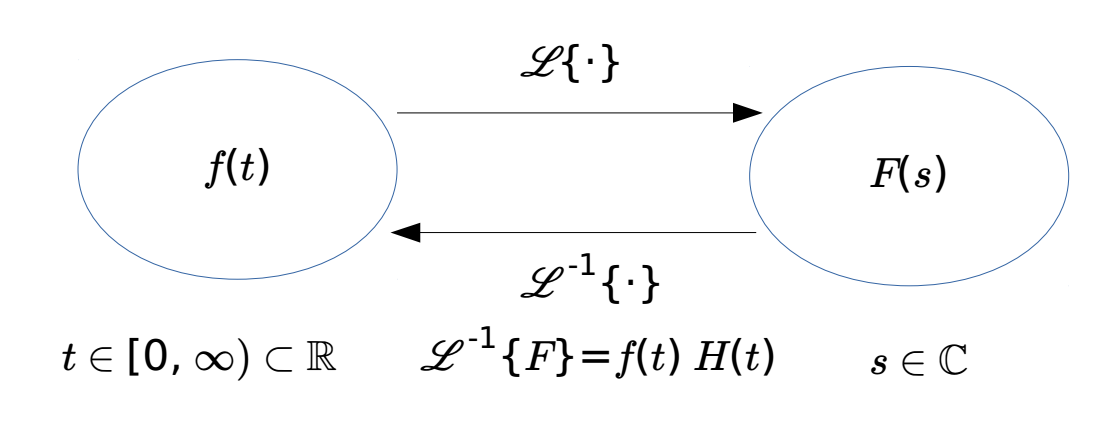
\includegraphics[scale=0.4]{diagrama.png}
\end{center}

\subsection*{El escal\'on unitario de Heaviside}
A continuaci\'on presentamos una funci\'on que nos ser\'a de bastante utilidad de ahora en adelante, y se conoce como la \textbf{funci\'on escal\'on unitario}, o \textbf{funci\'on escal\'on de Heaviside}. Se define como sigue:

\begin{equation*}
  H(t)=\begin{cases}
    1, & \text{si $t\geq 0$}.\\
    0, & \text{si $t<0$}.
  \end{cases}
\end{equation*}

Por c\'omo est\'a definida, deber\'ian reconocerla como una funci\'on causal: vale cero para cualquier $t$ menor que 0. Y no s\'olo eso, sino que para todo $t$ restante vale la unidad. Esto lo convierte por excelencia en la herramienta que nos permitir\'a convertir cualquier otra funci\'on $f(t)$ que no sea causal, en una que s\'i lo sea, con s\'olo multiplicarla por $H(t)$, de manera tal que le removemos la parte por detr\'as de $t=0$, y conservamos intacta la parte donde $t\geq 0$. De esta forma, nos garantizamos que para cualquier funci\'on real $f(t)$, se tiene que $f(t) H(t)$ \textbf{es causal}.

\begin{center}
	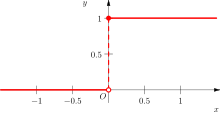
\includegraphics[scale=1]{HdeT.png}
\end{center}

Entonces, si tenemos una funci\'on $f(t):(-\infty, +\infty)\to \mathbb{R}\ \acute{o}\ \mathbb{C}$, tenemos que:

\begin{equation*}
  f(t)H(t)=\begin{cases}
    f(t), & \text{si $t\geq 0$}.\\
    0, & \text{si $t<0$}.
  \end{cases}
\end{equation*}

Y con ello hemos convertido a $f(t)$ a la causalidad. Am\'en.\\

Conocer a la funci\'on escal\'on de Heaviside es de suma importancia a la hora de calcular transformadas inversas, ya que toda funci\'on cuya transformada calculemos, se asumir\'a ser causal, y por consiguiente, toda trasnformada inversa que calculemos, \textit{nos deber\'a dar como resultado una funci\'on causal}. Y para darlo a entender, lo expresaremos de la forma $f(t)H(t)$, pudiendo ser $f(t)$ una funci\'on en donde se puede dar que $f(t)\neq 0,\ t<0$, pero eso ya no importar\'ia, ya que truncamos su comportamiento por detr\'as de $t=0$ al multiplicarla por la funci\'on de Heaviside.

\subsection*{La antitransformada: la definici\'on formal}
\textit{Dada la funci\'on de variable compleja $F(s)$, si existe $f(t)$ causal tal que $\mathscr{L}\{f(s)\} = F(s)$, entonces se denomina a $f(t)$ la \textbf{transformada inversa de Laplace} de $F(s)$ y se indica:}

\begin{center}
{\large$\mathscr{L}^{-1}\{F(s)\} = f(t)$}
\end{center}

\textit{En caso de que $f(t)$ no sea causal, entonces se define:}

\begin{center}
{\large$\mathscr{L}^{-1}\{F(s)\} = f(t)H(t)$}
\end{center}

Al operador $\mathscr{L}^{-1}\{\cdot\}$ se lo denomina operador de transformada inversa de Laplace.

\subsection*{Propiedades de la Transformada Inversa}
Para resolver las transformadas inversas de Laplace, nos complace deleitarlos con la siguiente simplicidad: como propiedades usaremos las mismas que detallamos para la Transformada de Laplace. Con ellas, buscaremos reconocer patrones para lograr armar la funci\'on causal que posea a $F(s)$ como su transformada. Mejor dicho, a encontrar $f(t)$, sea causal o no, ya que a la soluci\'on final la expresaremos siempre como $f(t)H(t)$.


\pagebreak
\section*{Resoluci\'on de EDOL a coeficientes constantes}

Se puede emplear la Transformada de Laplace y la Transformada Inversa de Laplace para encontrar las soluciones de Ecuaciones Diferenciales Ordinarias Lineales a Coeficientes Constantes, dadas las condiciones iniciales necesarias, para hallar la correspondiente \textit{soluci\'on particular}. Por este medio, no hallaremos ninguna soluci\'on general, sino que para aplicar este m\'etodo, necesitamos necesariamente las condiciones iniciales.



\end{document}